\chapter{Preliminaries}

Before we can discuss variants of the BFGS method, and quasi-Newton methods in general, we introduce certain basic principles and aspects, which will be needed later, in this section. The theoretical concepts have been taken from \cite{BerkolaikoKuchment:2013} where they are discussed in more detail and more background information can be found.

\section{Metric Graphs}

We define a graph $\Gamma$ as an ordered pair $(\mathcal{V}, \mathcal{E})$, where $\mathcal{V} = \{v_i\}$ is a finite or countably infinite set of points, which we call vertices, and $\mathcal{E} = \{e_j\}$ is a set of segments connecting some of the vertices, which we call edges. In the following we will use the notation $E \coloneqq \left\lvert \mathcal{E} \right\rvert$ for the number of edges and $E \coloneqq \left\lvert \mathcal{E} \right\rvert$ for the number of vertices. \\
A vertex $w \in \mathcal{V}$ is adjacent to a vertex $v \in \mathcal{V}$, denoted by $v \sim w$, if a suitable edge $e \in \mathcal{E}$ exists, so that $w$ can be reached from $v$ via this edge $e$. The notation $v \in e$ means that $v \in \mathcal{V}$ is a vertex of the edge $e \in \mathcal{V}$. In the following we assume that a graph has no loops, which are edges that connect a vertex to itself, i.e. $v \sim v$, and no multi-edges, which are several equal edges between two vertices. \\
A graph $\Gamma = (\mathcal{V}, \mathcal{E})$ is non-directed, if each of its edges $e \in \mathcal{E}$ connects two vertices $v, w \in \mathcal{V}$ and no direction is given to it. This means, if the vertices $v, w \in \mathcal{V}$ are connected by an edge $e \in \mathcal{E}$, that the vertex $v$ is adjacent to the vertex $w$, as well as the other way around, i.e. $w \sim v$ and $v \sim w$. A graph $\Gamma = (\mathcal{V}, \mathcal{E})$ is called directed graph, if each of its edges $e \in \mathcal{E}$ is assigned a direction, which means that each edge can only be followed in one direction. Therefore, the edges of a directed graph can be defined as ordered pairs of vertices , where the first vertex is called the origin vertex and the second vertex is called the end vertex of the corresponding edge. 

Directed edges will be called bonds. The set of all bonds is denoted by B. We will use the shorthand notation B := |B| for the total number of bonds in a directed graph Γ.
The order of the two connected vertices is unimportant.


Dies verdeutlicht, dass jede Kante des Graphen nur in eine Richtung durchlaufen werden kann.

Kanten in einem ungerichteten Graphen bezeichnet man als „ungerichtete Kanten“. Eine ungerichtete Kante ist demnach eine Menge von zwei Knoten. Mitunter wird der Begriff auch auf gerichtete Graphen ausgeweitet, um auszudrücken, dass zwei Knoten „a“ und „b“ sowohl durch die Kante {\displaystyle \left(a,b\right)}\left(a,b\right) als auch durch die Kante {\displaystyle \left(b,a\right)}\left(b,a\right) verbunden sind.

Kanten in einem gerichteten Graphen bezeichnet man als „gerichtete Kanten“. Sie besitzt also im Gegensatz zu einer ungerichteten Kante eine Orientierung. Für eine Kante {\displaystyle e=\left(a,b\right)}e=\left(a,b\right) wird der Knoten {\displaystyle a}a Startknoten und der Knoten {\displaystyle b}b Endknoten der Kante genannt. Eine gerichtete Kante wird auch „Bogen“ oder „Pfeil“ genannt. Zwei Kanten {\displaystyle e_{1}}e_{1}, {\displaystyle e_{2}}e_{2} mit {\displaystyle e_{1}=\left(a,b\right)}e_{1}=\left(a,b\right) und {\displaystyle e_{2}=\left(b,a\right)}e_{2}=\left(b,a\right) heißen „gegenläufig“ oder „antiparallel“.


Ist eine Verbindung zweier Knoten ein Pfeil, so ist der Graph gerichtet und die Kante darf nur in einer Richtung genutzt werden. Wie du siehst, ist es dir im gerichteten Graphen beispielsweise nicht erlaubt, vom Knoten B zum Knoten A zu gehen, da die Kante nur in die entgegengesetzte Richtung zeigt.

Wird eine Kante im Graphen hingegen als einfache Verbindung zwischen zwei Knoten dargestellt, ist der Graph ungerichtet und es muss nicht auf die Richtung geachtet werden.


On the other hand, in
most of the text graphs will be considered as 1D complexes, and thus
edges will be treated as 1D segments (or could be thought of as physical
“wires”). Such graphs will be equipped with additional structures that
will make them metric
\section{Drift-Diffusion Equations on Metric Graphs}
\label{ch1:sec2}

In this section, we introduce a model that uses a set of differential equations defined on the edges of a metric graph to represent the traffic flow in a road network. We want to solve this model in an approximate way later in the thesis using various methods. \\
We imagine a compact road network, where we mean a finite number of finitely long roads connected by a finite number of junctions. We note that in a realistic road network there also exist roads which simply end, i.e. roads which end in an junction to which no other roads are connected, and there exist also one-way roads between two junctions. To model such a compact road network, we identify it with a compact directed metric graph $\Gamma = (\mathcal{V}, \mathcal{E})$, where obviously the roads are identified by edges $e \in \mathcal{E}$ and the junctions $v \in \mathcal{V}$ by vertices. The length $\ell_e > 0$ of each edge $e \in \mathcal{E}$ is either given by the length of the associated road or some other isometric representation of it. An example of such a compact road network is illustrated in Figure 1 and the associated graph is illustrated in Figure 2. \\

\begin{figure}[H]
    \begin{subfigure}[b]{0.4\textwidth}
        \begin{center}
            \includegraphics[scale=0.4]{img/Kaßberg2.png}
        \end{center}
        \caption{Non-directed graph}
        \label{fig8:f1}
    \end{subfigure}
    \begin{subfigure}[b]{0.4\textwidth}
        \begin{center}
            \includegraphics[scale=0.15]{img/Kaßberg2-Darstellung.png}
        \end{center}
        \caption{Directed graph}
        \label{fig8:f2}
    \end{subfigure}
    \caption{Two different types of graphs.}
\end{figure}

There exist several approaches to model the traffic flow on a road network. One of the most important approaches was presented in \cite{LighthillWhitham:1955} and independently in \cite{Richards:1956}, in which the traffic flow is described by equations describing the flow of water. These fluid dynamics equations are a set of partial differential equations known as the Navier-Stokes equations, which express the conservation of mass, momentum, and energy. The basic idea of this approach is to look at large scales so to consider individual cars as small particles and a set of cars as mass, and their density as the main quantity to be considered. The model in this thesis is inspired by the same idea, which is why we focus on the density of cars on an individual edge $e \in \mathcal{E}$, which we want to model with a function $\rho_e \colon (0, T) \times [0, \ell_e] \to \mathbb{R}_{+}$, where $\rho_e (t,x)$ describes the concentration of some quantity, i.e. the density of cars, at the time $t \in (0, T)$ at the coordinate $x \in [0, \ell_e]$ on the edge $e \in \mathcal{E}$. It is reasonable to assume the conservation of the number of cars, which can be expressed by a continuity equation for each individual edge $e \in \mathcal{E}$
\begin{equation}
    \label{continuity equation}
    \partial_t \rho_e (t,x) = - \partial_x J_e(t,x),
\end{equation}
where $J_e \colon (0,T) \times [0, \ell_e] \to \mathbb{R}$ is the flux of cars. \cref{continuity equation} describes the transport of a certain quantity of cars and expresses a relationship between the density of cars and the flux by linking the temporal change of the density to the spatial change of its flux density with the assumption of conservation of the number of cars. \\
Let the flux in the model in this thesis be given by 
\begin{equation} 
    \label{eq:flux} 
    J_e(t,x) \coloneqq - \varepsilon \partial_x \rho_e (t, x) + f(\rho_e(t, x)) \partial_x V_e(t, x).
\end{equation}
The flux is composed of two terms. The first term, $- \varepsilon \partial_x \rho_e (t, x)$, describes the transport by diffusion, which is given by Fick's first law, see \cite{Fick:1855}, where $\varepsilon > 0$ is the so-called diffusion coefficient. The second term, $f(\rho_e(t, x)) \partial_x V_e(t, x)$, describes the transport by flow or drift, where $V_e \colon (0,T) \times [0, \ell_e] \to \mathbb{R}_{+}$ is a given potential, that may vary from edge to edge, the function $f \colon \mathbb{R}_{+} \to \mathbb{R}_{+}$ is called mobility and its simplest choice is the so-called linear transport $f(\rho_e) = \mathrm{v} \cdot \rho_e$ with $\mathrm{v}$ the average velocity of cars. However, in many applications, the density $\rho_e (t,x)$ is not allowed to exceed a maximal value $\rho_{e, max}$ (e.g. due to finite size effects). In the model in this thesis it is required that the mobility $f$ satisfies $f(0) = f(\rho_{e, max}) = 0$. If this value is scaled to one, a choice of $f$ that obeys $f(0) = f(1) = 0$, such as $f(\rho_e) = (1-\rho_e) \rho_e$, will ensure that solutions to \eqref{continuity equation} will satisfy this bound for all time. The choice of $f(\rho_e) = (1-\rho_e) \rho_e$ is quite common, since the average velocity $\mathrm{v}$ is often considered as a function of $\rho_e$ and the linear decreasing function $\mathrm{v} = \mathrm{v}_{max} (1-\rho_e)$ is often chosen for it. The model in this thesis follows this approach, but we set $\mathrm{v}_{max} = 1$. We note that with this choice of $f$ it follows that all edges in the graph $\Gamma$ must be directed, because by defining the flux $J_e(t,x)$ via \cref{eq:flux} we consider first order derivatives in the continuity equation, see \cref{continuity equation}, on the graph $\Gamma$ and we need directions for first order derivatives. We further note that the derivative in $J_e(t,x)$ is taken into the outgoing direction. \\

Summarized, the model is posed on a compact directed metric graph $\Gamma = (\mathcal{V}, \mathcal{E})$, where each edge $e \in \mathcal{E}$ is equipped with a length $\ell_e > 0$ and the differential equation
\begin{equation} 
    \label{Drift-Diffusion-equation}
    \partial_t \rho_e (t,x) = \partial_x (\varepsilon \partial_x \rho_e (t,x) - f(\rho_e (t,x) ) \partial_x V_e (t,x)),
\end{equation}
where $\rho_e \colon (0, T) \times [0, \ell_e] \to [0, 1]$ is the searched function, $\varepsilon > 0$ is a constant, $V_e \colon (0,T) \times e \to \mathbb{R}_{+}$ is a given potential and $f \colon \mathbb{R}_{+} \to \mathbb{R}_{+}$ is a function, that satisfies $f(0) = f(1) = 0$. From now on, we refer to the differential equation given by \cref{Drift-Diffusion-equation} as drift-diffusion equation. \\
To make \cref{Drift-Diffusion-equation} a well-posed problem, we need to add initial-conditions as well as coupling conditions on the vertices. For that we denote the ordered pair of vertices connected by a directed edge $e \in \mathcal{E}$ by $(v^{o}_e, v^{t}_e)$ and define a normal vector $n_e$ to each edge $e = (v^{o}_e, v^{t}_e)$ via $n_e(v^{o}_e) = -1$ and $n_e(v^{t}_e) = 1$. \\
On the set of interior vertices $v \in \mathcal{V}_\mathcal{K} \subset \mathcal{V}$, which are vertices that are incident to at least one incoming edge and at least one outgoing edge (i.e.$\forall v \in \mathcal{V}_\mathcal{K} \; \exists \ e_1, e_2 \in \mathcal{E}$ such that $v^{t}_{e_1} = v$ and $v^{o}_{e_2} = v$), we apply homogeneous Kirchhoff-Neumann coupling conditions, i.e. on each $v \in \mathcal{V}_\mathcal{K}$ holds
\begin{equation}
    \label{eq:Kirchhoff_Neumann_condition}
    \sum_{e\in \mathcal{E}_v} J_e(t,v) n_e (v)=0,
\end{equation}
where $\mathcal{E}_v$ is the edge set incident to the vertex $v$. Additionally, we ask the solution of \cref{Drift-Diffusion-equation} to be continuous on the set of interior vertices, i.e. 
\begin{equation}
    \label{continuous on vertices}
    \rho_e(v) = \rho_{e'}(v) \quad \text{ for all }v \in \mathcal{V}_\mathcal{K},\; e,\,e' \in \mathcal{E}_v.
\end{equation}
On the set of exterior vertices $v \in \mathcal{V}_\mathcal{D} \coloneqq \mathcal{V} \setminus \mathcal{V}_\mathcal{K}$, which are vertices that are incident to either only one incoming edge or only one outgoing edge (i.e. $\forall v \in \mathcal{V}_\mathcal{D} \; \exists! \ e \in \mathcal{E}$ such that either $v^{t}_{e} = v$ or $v^{o}_{e} = v$), the solution $\rho$ should fulfills the flux boundary conditions
\begin{equation}
    \label{eq:Dirichlet_conditions}
    \sum_{e\in \mathcal{E}_v}J_e(v) n_e (v)=-\alpha_v(t) (1-\rho_v) + \beta_v(t) \rho_v,\ \text{for all}\ v \in \mathcal{V}_\mathcal{D}, e \in \mathcal{E}_v,
\end{equation}
where $\alpha_v \colon (0,T) \to \mathbb{R}_{+}$ prescribes the rate of influx of mass into the network and $\beta_v \colon (0,T) \to \mathbb{R}_{+}$, ${v \in \mathcal{V}_\mathcal{D}}$ prescribes the velocity of mass leaving the network at the exterior vertices ${v \in \mathcal{V}_\mathcal{D}}$. Note that this choice ensures that the bounds $0 \leq \rho_e \leq 1$ are preserved. In typical situations, exterior vertices are either of influx- or of outflux type, i.e. $\alpha_v(t) \beta_v(t) \equiv 0$ for all $v \in \mathcal{V}_\mathcal{D}$ for all $t \in (0,T)$. \\
The Kirchhoff-Neumann conditions are the natural boundary conditions for the differential equation \eqref{eq:Hamiltonian}, since they ensure, on the one hand, that exactly as much mass flows into each interior vertex $v \in \mathcal{V}_{\mathcal{K}}$ as flows out of it and, on the other hand, together with the the flux boundary conditions, \cref{eq:Dirichlet_conditions}, they ensure that mass enters or leaves the system only via the exterior vertices $\mathcal{V}_\mathcal{D}$ for which either $\alpha_v(t)$ or $\beta_v(t)$ is positive. \\
Finally, we impose an initial condition on each edge via 
\begin{equation}
    \label{eq:initial_conditions}
    \rho_e(0,x) = \rho_{e, 0}(x),
\end{equation}
where $\rho_{e, 0} \in L^2(e)$ returns the density on each point of the edge $e$ at time $t=0$. \\ 



We note that by \cref{Drift-Diffusion-equation} we obtain the following differential operator defined on the metric graph $\Gamma$
\begin{equation} 
    \label{eq:Hamiltonian}
    \mathcal{H} [\rho_e] (t,x) \coloneqq \partial_t \rho_e (t,x)  - \partial_x (\varepsilon \partial_x \rho_e (t,x) + f(\rho_e (t,x) ) \partial_x V_e (t,x))
\end{equation}
and together with the above mentioned initial and boundary conditions we obtain a triple which satisfies the definition of a quantum graph, see \cref{quantum graph}. Nevertheless, in the rest of this thesis we will refer to this approximation problem as drift-diffusion equations on a metric graph. 







\begin{theorem} 
    Given initial data $\rho_0 \in L^2(\Gamma)$ s.t. $0 \le \rho_0 \le 1$ a.e. on $\mathcal{E}$, there exists a unique weak solution $\rho \in L^2(0,T; H^1(\Gamma)) \cap H^1(0,T; (H^1)^*(\Gamma))$ s.t.
	\begin{align*}
		\sum_{e \in \mathcal{E}} \left(\int_e  \partial_t \rho_e \varphi_e \;dx + \int_e \partial_x \rho_e\partial_x \varphi_e \;dx\right) + \sum_{v \in \mathcal{V}_D} (-\alpha_v(t) (1-\rho_v) + \beta_v(t) \rho_v)\varphi(v) = 0,
	\end{align*}
	for all test functions $\varphi \in H^1(\Gamma)$.
\end{theorem}

%Kirchhoff: alles was in den Knoten reinfließt muss auch rausfließen
% Kirchhoff: We note that the derivative is taken into the outgoing direction.
%operator nicht selbstadjungiert
% graph muss gerichtet sein, ansosnten erste ableitung nicht möglich
% initial conditions übernehmen
% Analytische Lösung nicht möglich

\section{Neural Networks as Function Approximators}
\label{ch1:sec3}

Artificial intelligence refers to a branch of computer science that deals with the automation of intelligent behaviour, which can be understood as the intelligence displayed by machines. Artificial intelligence further refers to the attempt to emulate certain decision-making structures of humans by, for example, building and programming a computer in such a way that it can handle problems relatively independently. Today, artificial intelligence is a thriving field with many practical applications and active research topics. Many applications involve deriving a general rule from a set of data, which is called machine learning. Artificial intelligence has recently made great progress in the field of artificial neural networks, which are roughly inspired by the structure of the human brain, are artificially simulated on the computer and can be used as universal function approximators. \\
In this section we describe artificial neural networks, usually just called neural networks, which are computing systems inspired by the biological neural networks that constitute human brains. The original objective of the research field of artificial intelligence was to solve problems in the same way as the human brain would do, using a neural network approach. Today, neural networks can be used to model complex relationships between inputs and outputs or to find patterns in data. It has been shown that these systems can be used very well as classifiers as well as regressors or function approximators. \\
An artificial neural network is a collection of interconnected units called artificial neurons or just neurons that replicate biological neurons in a human brain, which are special cells in the nervous system that transmit information to other neurons through synapses. Each connection, like the synapses in a human brain, can transmit information, which can be understood as a signal, from one artificial neuron to another. The receiving neuron can process the signal, or even the signals, and then transmit signals to the downstream neurons that are connected to it. In common neural network types, the signal at a connection between artificial neurons is a real number, and the output of each artificial neuron is calculated by a non-linear function of the weighted sum of its inputs. Artificial neurons and their connections usually have a weight that changes during a learning process. The weight increases or decreases the strength of the signal at a connection, where a positive weight represents an excitatory connection, while a negative weight represents an inhibitory connection. \\
However, artificial neural networks are more about an abstraction of that information processing, less about replicating biological neurons or human brains. In 1958, the psychologist Frank Rosenblatt invented the first mathematical model for a single neuron, termed perceptron, in \cite{Rosenblatt:1958}, which was also the first artificial neural network. We want to use artificial neurons based on the perceptron and the neural networks constructed from them to approximate a variety of functions. \\
Let us describe how a single artificial neuron transforms a real-valued input into a 1-dimensional output, as illustrated in \cref{fig4}. Let there be $n$ real-valued input values summarized in a vector $(x_1, \ldots, x_n)^{\mathrm{T}} = x \in \mathbb{R}^n$. First, one forms a biased and weighted sum with the input values $x_1, \ldots, x_n$, which is nothing other than a linear combination, i.e. 
\begin{equation*}
    a = \sum^{n}_{i=1} w_i x_i + b = w^{\mathrm{T}} x + b,
\end{equation*}
where $(w_1, \ldots, w_n)^{\mathrm{T}} = w \in \mathbb{R}^n$ are called weights and $b \in \mathbb{R}$ is called bias. These weights and the bias are either predetermined or learned by the neuron itself through data (machine learning), but more on that later. The linear combination $a$ is called activation in the context of neural networks and a so-called activation function $\sigma \colon \mathbb{R} \to \mathbb{R}$ is applied to it, so that the output of that neuron becomes
\begin{equation*}
    y = \sigma \left( \sum^{n}_{i=1} w_i x_i + b \right) = \sigma \left( w^{\mathrm{T}} x + b \right) = \sigma(a).
\end{equation*}

\begin{figure}[H]
    \begin{center}
        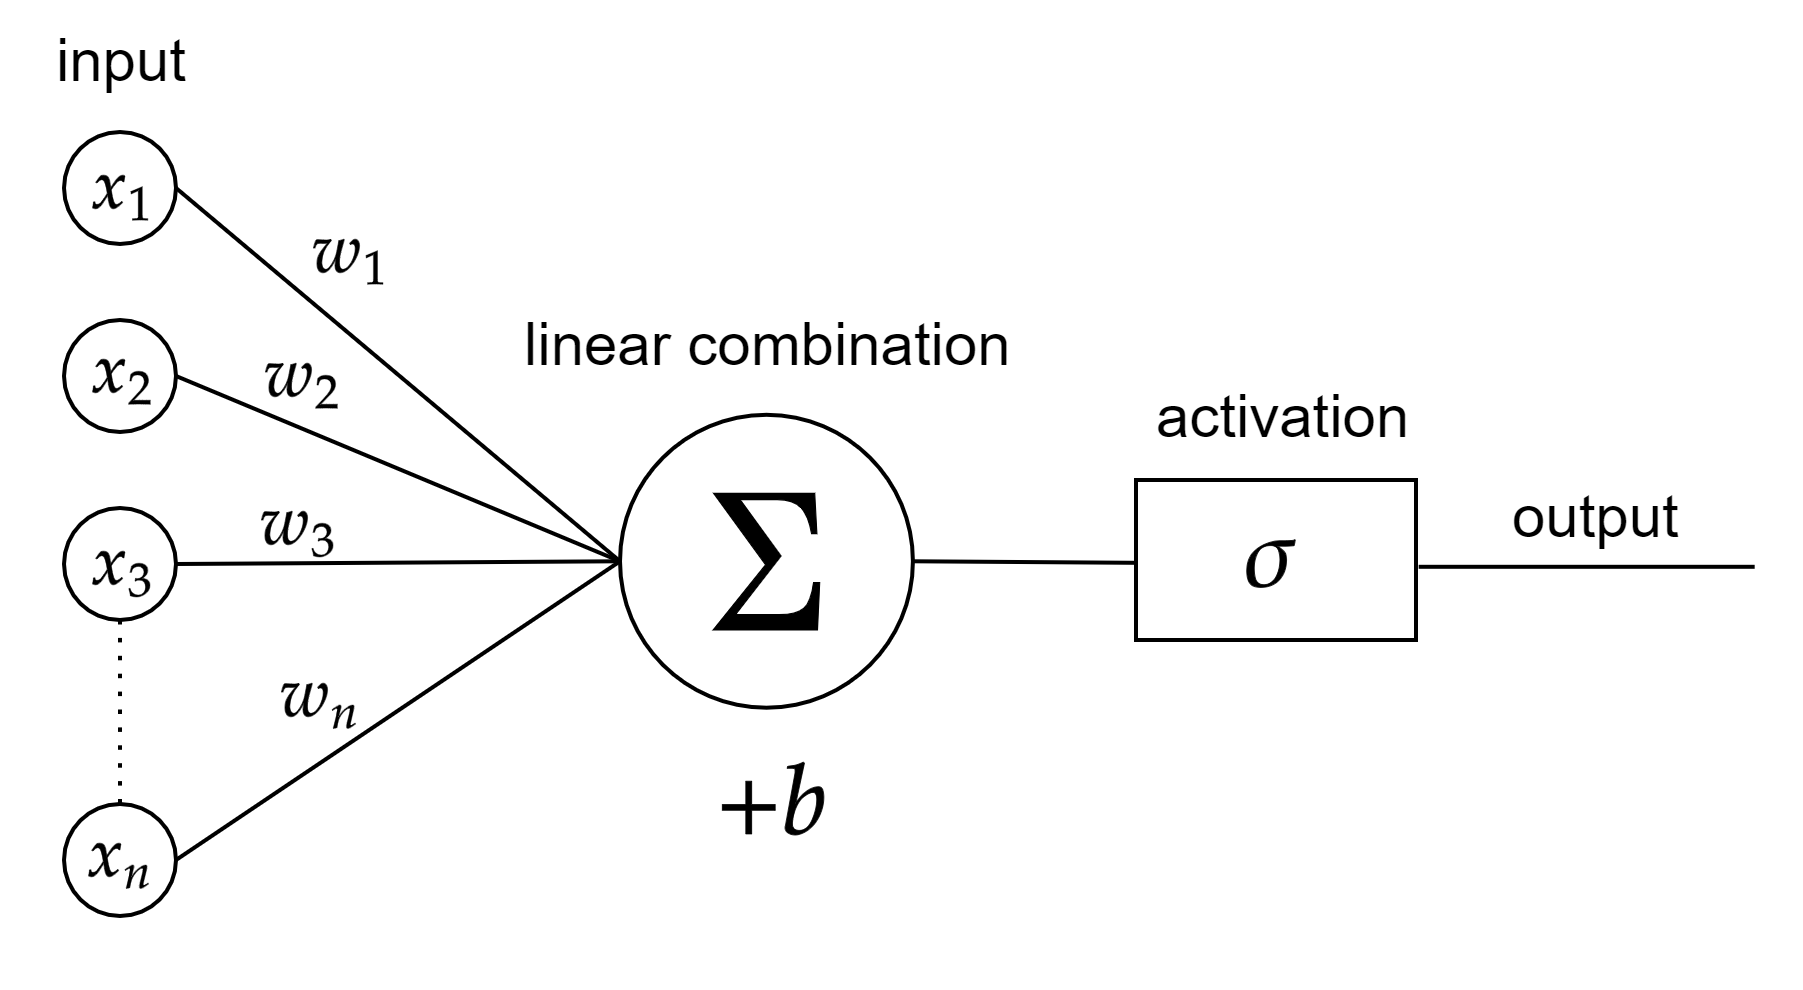
\includegraphics[scale=0.25]{img/diagram-20220205_1.png}
    \end{center}
    \caption{Illustration of the mathematical model of a single artificial neuron.}
    \label{fig4}
\end{figure}

The choice of activation function is determined by the nature of the input and the assumed distribution of the output. When the activation function is for example equal to the Heaviside step function, as described in \cite{Rosenblatt:1958}, i.e.
\begin{equation*}
    \sigma(x) = \begin{cases} 1 & \text{if } x \geq 0, \\ 0 & \text{if } x < 0, \end{cases}
\end{equation*}
then the artificial neuron coincides with a so-called linear support vector classifier, which is a mathematical method of pattern recognition that divides a set of objects into classes in such a way that the widest possible area around the class boundaries remains free of objects, see \cite[Chapter~7]{Bishop:2006}. \\
The task of the activation function is only to turn the linear combination of the input $a$ into a non-linear output $\sigma(a)$. Therefore, any non-linear, non-constant function can be an activation function, but those generally used are additionally monotone increasing, continuous, and at least piecewise smooth. At present, the most popular activation function is the rectified linear unit, abbreviated ReLU, \cref{ReLU}. In recent decades, smoother activation functions have also been used, such as the sigmoid function, \cref{Sigmoid}, or the hyperbolic tangent function, \cref{TanH}, \cite[p.~3]{LeCunBengioHinton:2015}.
\begin{align}
    \sigma(y) &=\max \{y, 0\} & & \text{ rectified linear unit (ReLU) } \label{ReLU} \\
    \sigma(y) &=\frac{1}{1+\exp (-y)} & & \text{ sigmoid } \label{Sigmoid} \\
    \sigma(y) &=\tanh (y)=\frac{\exp (y)-\exp (-y)}{\exp (y)+\exp (-y)} & & \text{ hyperbolic tangent } \label{TanH}
\end{align}

Unfortunately, a single neuron is incapable of both producing a multi-dimensional output and approximating any reasonably complicated function. This led to the creation of networks of artificial neurons, known as (artificial) neural networks. There are many different types of neural networks, which differ in their so-called architecture, which specifies how the neurons are organised, what activation functions are used and what other mathematical operations occur. Often a certain type of neural network is particularly suitable for a specific problem to be solved. A combination of different networks for solving a problem is also possible. \\
In the following, we focus on the best known and one of the most important types of neural networks, which form a specific class of neural networks that have proven most effective in practice, namely (deep) feed-forward neural networks, abbreviated FNNs. In these neuronal networks, the neurons are organized in multiple layers and neurons of one layer connect only to neurons of the immediately following layer. This means that the outputs of the neurons of one layer is utilized as inputs to the neurons of the following layer. This also describes the term feed-forward, which means that the information only flows in one direction, forwards. There are no backward connections in which outputs of one layer are fed back into itself. When FNNs are extended to include backward connections, they are called recurrent neural networks. Between the neurons of two layers, multiple connection patterns are possible. FNNs are in general fully connected, which means that the output of each neuron in one layer would be passed to all neurons in the following layer. FNNs are also known as multilayer perceptrons, although this name can be misleading as the artificial neurons are usually not the perceptrons as introduced in \cite{Rosenblatt:1958}. \\
We now describe how FNNs can be modelled in mathematical terms. We assume that we have $L \in \mathbb{N}$ layers of artificial neurons. We use $n_l \in \mathbb{N}$ to denote the number of neurons in layer $1 \leq l \leq L$. These numbers describe the topology of an FNN, the number of layers is called depth and the maximum number of neurons in a layer is called width of an FNN. This is why we also speak of deep feed-forward networks, as they can often have multiple layers. \\
To simplify the notation of FNNs, we introduce a so-called input layer with $l=0$, which only receives the external data $x$. It is the first layer of the network and does not change the input $x$ in any way. The number of neurons in this layer corresponds to the dimension of the input, i.e. $x \in \mathbb{R}^{n_{0}}$. From now on, we will refer to the last layer $l = L$ of a FNN, which produces the ultimate result, as the output layer. The number of neurons in this layer is equal to the dimension that the desired output should have, i.e. $y \in \mathbb{R}^{n_{L}}$. If an FNN has more than one layer, i.e. $L>1$, we refer to all layers between the input layer and the output layer as hidden layers. If the FNN does not have one hidden layer, it is called a single layer network because only the output layer $L=1$ processes the information. \\
We consider the information processing of a single layer $1 \leq l \leq L$. As input, each of the $n_l$ neurons in layer $l$ receives the output $x^{l-1} \in \mathbb{R}^{n_{l-1}}$ of the $n_{l-1}$ neurons in the previous layer $l-1$. Each neuron in layer $l$ has its own weight vector $w_i \in \mathbb{R}^{n_{l-1}}$, $i = 1, \ldots, n_l$. The weights of all $n_l$ neurons in layer $l$ can be conveniently organized into a matrix $W^l \in \mathbb{R}^{n_l \times n_{l-1}}$, where the $i$-th row is the transposed weight vector, $w^{\mathrm{T}}_i$, of the $i$-th neuron. We summarize the $n_l$ biases of the $n_l$ neurons into a vector $b \in \mathbb{R}^{n_l}$. The input $x^{l-1}$ is now linearly combined $n_l$ times with the weights and biases of the $n_l$ neurons of layer $l$ via 
\begin{equation}
    \label{propagation function}
    a^l = W^l x^{l-1} + b^l \in \mathbb{R}^{n_l}.
\end{equation}
We call \cref{propagation function} propagation function of layer $l$. \\
The same activation function is used in all neurons of layer $l$, which is why we define the activation function $\sigma \colon \mathbb{R} \to \mathbb{R}$ for vector-valued input values $a \in \mathbb{R}^{n_l}$ by applying it component-wise:
\begin{equation*}
    \sigma_l \colon \mathbb{R}^{n_l} \ni a^l \mapsto \sigma_l (a^l):= \left(
        \begin{array}
            {c} \sigma_l \left( a^l_{1} \right) \\
            \vdots \\
            \sigma_l \left( a^l_{n_l} \right)
        \end{array}
        \right) \in \mathbb{R}^{n_l}.
\end{equation*}
We note that the activation function $\sigma_l$ can vary from layer to layer, which is why we indicate the dependency with the index $l$. The complete transformation of the input $x^{l-1} \in \mathbb{R}^{n_{l-1}}$ in the $l$-th layer can then be written as
\begin{equation}
    \label{action layer}
    \mathbb{R}^{n^{l-1}} \ni \underbrace{x^{l-1}}_{\text{input of layer } l} \mapsto x^{l}:=\underbrace{\sigma_{l}\left( W^{l} x^{l-1} + b^{l} \right)}_{\text{output of layer } l}=: f^{l}_{\theta_l} \left( x^{l-1} \right) \in \mathbb{R}^{n^{l}}, 
\end{equation}
where $\theta_l = (W^{l}, b^{l})$. \\

\begin{figure}[H]
    \begin{center}
        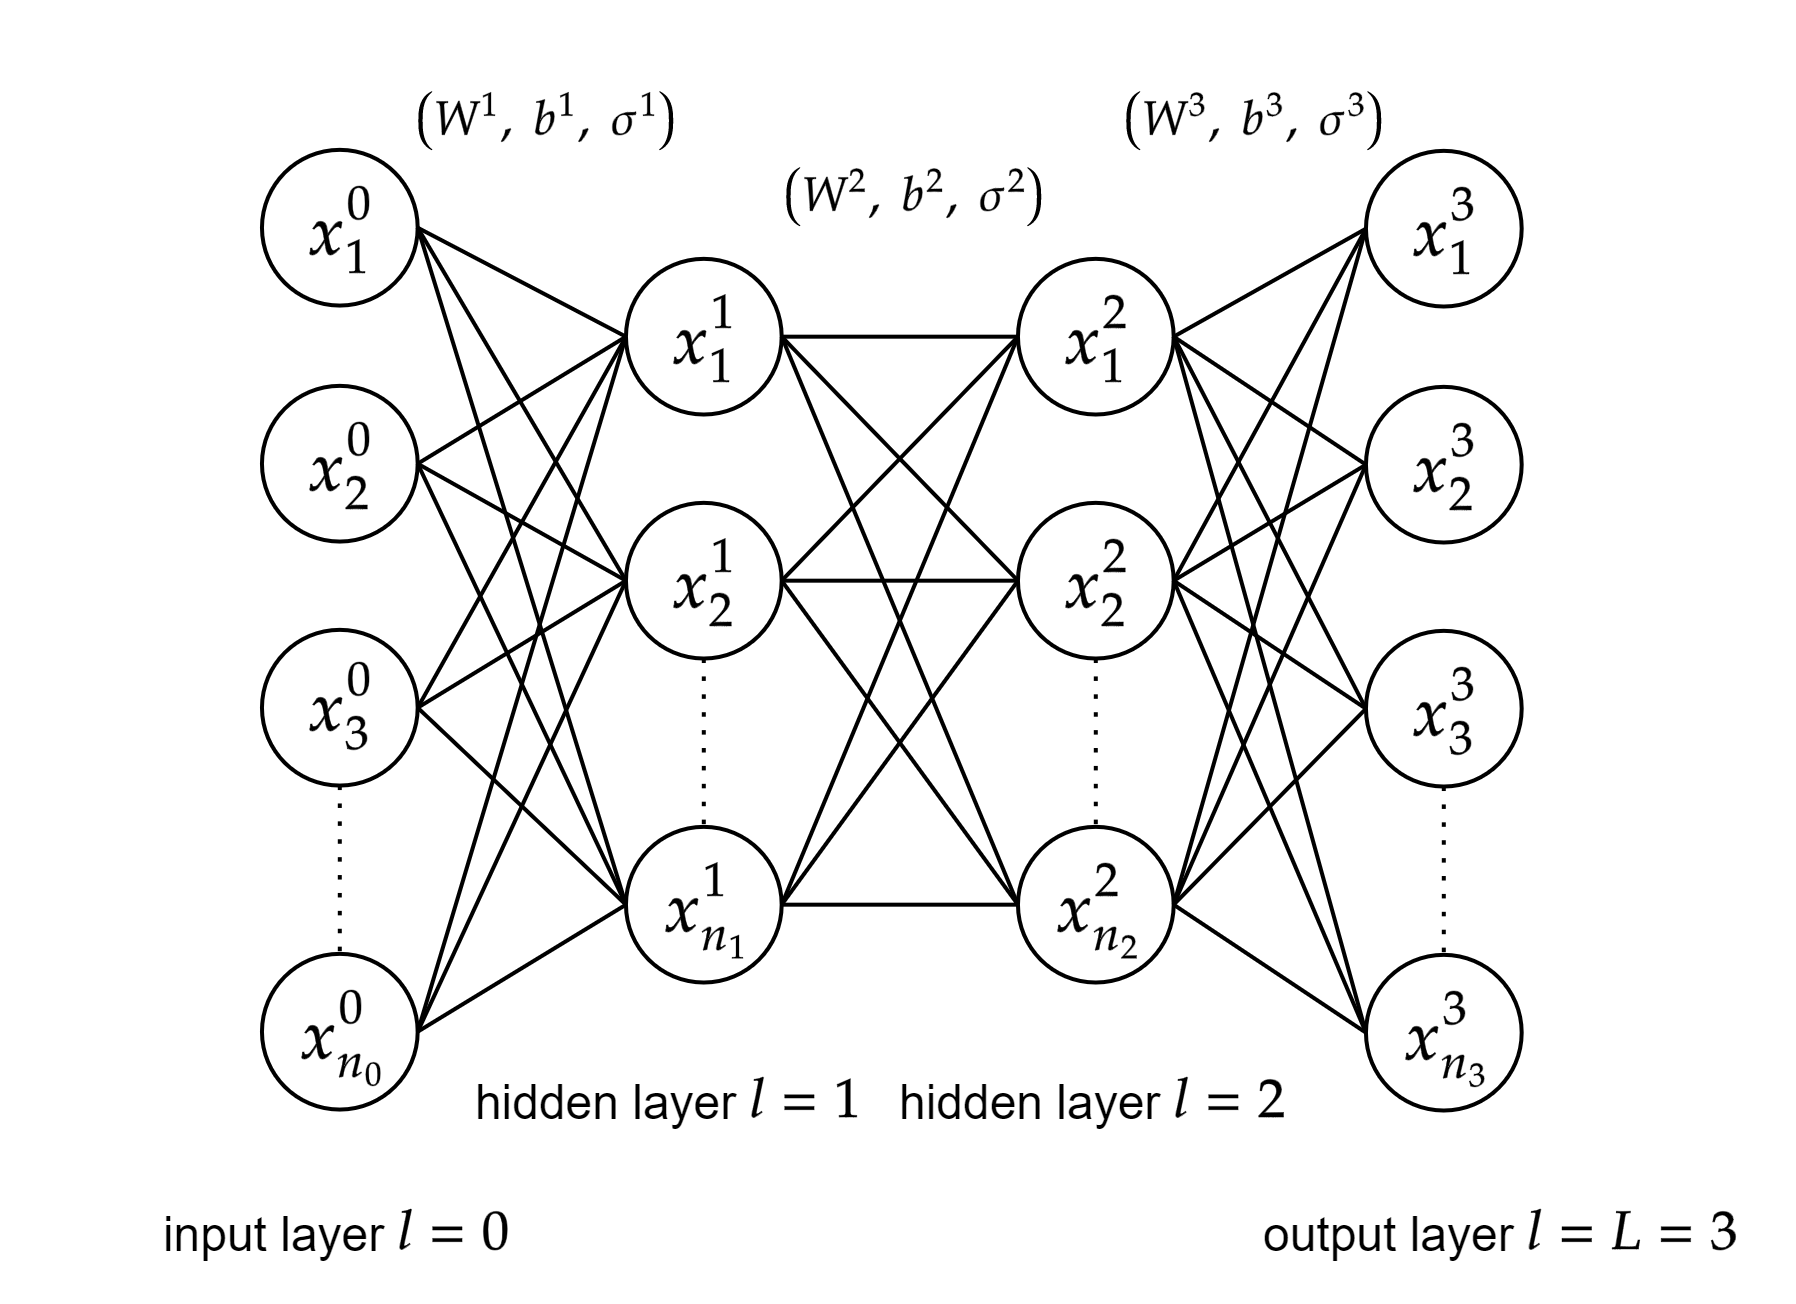
\includegraphics[scale=0.25]{img/diagram-20220206.png}
    \end{center}
    \caption{Illustration of a feed-forward neural network with $L=3$ layers.}
    \label{fig5}
\end{figure}

A feed-forward neural network consists of a composition of several of these layer-wise actions, \cref{action layer}, which are executed one after the other. Therefore, FNNs can be well represented as a directed acyclic graph (a directed graph with no directed cycles. We omit the arrows at the edges, since the flow direction of the information is in general always known.), where the neurons are represented as vertices and the connections of the neurons are represented as edges. The input layer $l=0$ is sometimes also represented as a layer of vertices. An example of an FNN is illustrated in \cref{fig5}, where the FNN has $L=3$ layers and therefore $2$ hidden layers. The mapping of the input $x = x^0 \in \mathbb{R}^{n_0}$ to the output $y = x^3 \in \mathbb{R}^{n_3}$ by the FNN is given by 
\begin{equation}
    \label{forward propagation of information}
    \begin{aligned}
        x^3 &=\sigma_{3} \left( W^{3} \sigma_{2} \left(  W^{2} \sigma_{1} \left( W^{1} x^{0}+b^{1}\right)+b^{2}\right)+b^{3}\right) \\
        & =f^{3}_{\theta_3} \left( f^{2}_{\theta_2} \left( f^{1}_{\theta_3} \left(x^{0} \right) \right) \right) \\
        & = f_{\theta} \left( x^{0}\right). \\
    \end{aligned}
\end{equation}
The process \cref{forward propagation of information} is called model prediction of the corresponding neural network and can be interpreted as a forward propagation of information through the layers of the network. In the following, we will identify the model prediction of a neural network with the subscript $\theta$, which constitutes the summary of all weights and biases (and other network-dependent parameters) of the network under consideration, i.e. $\theta = (W,b)$ with $W = \{ W^l \}_{l = 1, \ldots, L}$ and $b = \{ b^l \}_{l = 1, \ldots, L}$. From \cref{forward propagation of information} it is clear that the activation functions $\sigma_l$ should be non-linear. Otherwise, the output $x^L$ is a linear function of the input $x^0$ and all layers could be combined into one output layer. \\

We have seen how a FNN produces a non-linear multidimensional output from a multidimensional input. For a network to solve a problem such as approximating a function $f \colon \mathbb{R}^n \to \mathbb{R}^m$, the weights $W$ and biases $b$ need to be properly adjusted. This is what machine learning deals with, which is one of the largest areas of artificial intelligence. Machine learning is a generic term for the artificial generation of knowledge from experience: a neural network learns from examples that are given as a data set and can generalise them after a so-called learning phase. Neural networks do not simply learn the examples, but recognise patterns and regularities in the data. Deep learning is part of a broader family of machine learning methods that uses deep neural networks, abbreviated DNNs, to build out a comprehensive internal structure so that complex non-linear relationships can be modelled. DNNs are usually FNNs with a very high depth, i.e. with numerous hidden layers that perform different types of transformations on their input. The more complex the problem to be solved with the help of the neural network is, the more layers are needed. This number of many layers means that a lot of parameters, which are the entries of the weight matrices $W^l \in \mathbb{R}^{n_l \times n_{l-1}}$ and of the bias vectors $b^l \in \mathbb{R}^{n_l}$, have to be modified in a FNN, that is
\begin{equation*}
    \underbrace{n_0 \cdot n_1 + \ldots + n_{L-1} \cdot n_L}_{\text{weights}} + \underbrace{n_0 + \ldots + n_L}_{\text{biases}}.
\end{equation*}
The learning through data of these deep networks is called deep learning. Machine learning approaches are traditionally divided into three major categories, depending on the type of data available to the neural network: supervised learning, unsupervised learning and reinforcement learning. We focus on the first two. \\
Suppose we want to approximate a map
\begin{equation*}
    f \colon \mathbb{R}^n \to \mathbb{R}^m
\end{equation*}
with a FNN. In an supervised learning approach, it is assumed that a so-called training data set $\{ (x_i, y_i) \}_{i = 1, \ldots, N}$ is given, consisting of ordered pairs of inputs $x_i \in \mathbb{R}^n$ and desired output values $y_i \in \mathbb{R}^m$ of the function $f$ to be approximated, i.e. $y_i = f(x_i)$. The idea of supervised learning is to confront the neural network $f_{\theta}$, which is to approximate the function $f$, with the correct function value $y_i$ for an input value $x_i$. The goal is to train the neural network $f_{\theta}$ to make associations after several computations with different inputs $x_i$ and outputs $y_i$, so that the network $f_{\theta}$ approximates the function $f$ well to a certain degree. For this purpose, a cost function is defined that compares the desired output values $y_i$ with the outputs produced by the network $f_{\theta}(x_i)$ with the corresponding inputs $x_i$. This is generally achieved by using the so-called mean squared error, abbreviated $MSE$, which is the average squared difference between the generated values $f_{\theta}(x_i)$ and the actual values $y_i$. One then tries, with the help of a learning algorithm, to choose the weights and biases $\theta = (W, b) = (\{ W^l \}, \{ b^l \})_{l = 1, \ldots, L}$ such that the $MSE$ can be kept as small as possible over all data pairs $\{ (x_i, y_i) \}_{i = 1, \ldots, N}$. This can be defined as the following optimization problem:
\begin{equation}
    \label{supervised learning}
    \begin{gathered}
        \text{ Minimize } \underbrace{\frac{1}{N}}_{\text{normalization factor}} \sum_{i=1}^{N} \lVert \underbrace{ f_{\theta} \left(x_{i}\right)}_{\text{model prediction }} - \underbrace{y_{i}}_{\text{actual data }} \rVert^{2}_2 =  MSE(\{ (x_i, y_i) \}_{i = 1, \ldots, N}, \theta) \\
        \\
        \text{ where } \; \theta = (\{ W^l \}, \{ b^l \})_{l = 1, \ldots, L}, \; \; \left(W^{l}, b^{l}\right) \in \mathbb{R}^{n_l \times n_{l-1}} \times \mathbb{R}^{n_l}, \; \; l=1, \ldots, L .
    \end{gathered}
\end{equation}
\cref{supervised learning} is called a non-linear least-squares optimization problem. It is an unconstrained problem whose objective is generally non-convex. Of course, loss functions other than the $MSE$ can be used, but the $MSE$ has become the most common because of the differentiability it provides. \\
In an unsupervised learning approach, a training dataset is given only with input values, i.e. $\{ x_i \}_{i = 1, \ldots, N}$. In this machine learning approach, the networks try to recognise structures in the given input data. The networks therefore learn from data that has not been categorised in any way. Instead of responding to feedback, unsupervised learning methods identify commonalities in the data and respond based on the presence or absence of such commonalities. There are several methods of unsupervised learning. Again, there is the possibility of defining a cost function, which is passed an input value $x_i$ and the output generated by the network $f_{\theta}(x_i)$. The cost function depends on the problem and all a priori assumptions for the function $f$ to be approximated. However, a cost function can be very complicated, as its form depends on the problem at hand. One can again take the approach from \cref{supervised learning} and try to minimize the mean value of the cost function evaluated over all training inputs $\{ x_i \}_{i = 1, \ldots, N}$ and the output values generated by the network $\{ f_{\theta}(x_i) \}_{i = 1, \ldots, N}$ with respect to the weights $\{ W^l \}_{l = 1, \ldots, L}$ and biases $\{ b^l \}_{l = 1, \ldots, L}$. The unsupervised learning approach offers the advantage that only the input values must be available, which can be the case for many approximation problems. \\

Of course, the optimization problem \cref{supervised learning} is not solved directly, but gradient-based optimization methods are generally used for this (which is why the term gradient-based learning is used for it, see e.g. \cite[p.~177]{GoodfellowBengioCourville:2016}), such as the variants of the gradient descent method. These are iterative methods that approximate a solution of \cref{supervised learning}, simply expressed via 
\begin{equation}
    \label{Gradient Descent}
    \theta_{k+1} = \theta_k - t \cdot \nabla_{\theta_k} \left( \frac{1}{N}\sum_{i=1}^{N} \lVert f_{\theta_k} \left(x_{i}\right) - y_{i}\rVert^{2}_2 \right) = \theta_k - t \cdot \nabla_{\theta_k} MSE(\{ (x_i, y_i) \}_{i = 1, \ldots, N}, \theta_k),
\end{equation}
where $\theta_k \in \prod^L_{l=1}  \mathbb{R}^{n_l \times n_{l-1}} \times \mathbb{R}^{n_l}$ are the iterations in the search space and $t > 0$ is the so-called learning rate, which can either be given or calculated with the help of a line search method. In many cases the data set $\{ (x_i, y_i) \}_{i = 1, \ldots, N}$ is very large and because of the linearity of differentiation and because the gradient $\nabla_{\theta_k} MSE(\{ (x_i, y_i) \}_{i = 1, \ldots, N}, \theta_k)$ also consists of many components, one for each $W^l$ and $b^l$, an ordinary gradient descent method may be too exhaustive to use. This is remedied by the stochastic gradient descent method, abbreviated SGD, in which $\nabla_{\theta_k} MSE(\{ (x_i, y_i) \}_{i = 1, \ldots, N}, \theta_k)$ is approximated by the gradient evaluated at only one data pair $(x_j, y_j)$, which is randomly selected from $\{ (x_i, y_i) \}_{i = 1, \ldots, N}$ with uniform distribution, i.e. $\nabla_{\theta_k} MSE((x_j, y_j), \theta_k)$ is used as direction in \cref{Gradient Descent}. An extension of this is the so-called mini-batch SGD method, in which $\nabla_{\theta_k} MSE(\{ (x_i, y_i) \}_{i = 1, \ldots, N}, \theta_k)$ is approximated by the gradient evaluated at a randomly selected small subset  of the data $\{ (x_i, y_i) \}_{i = 1, \ldots, J} \subsetneq  \{ (x_i, y_i) \}_{i = 1, \ldots, N}$ with $J \ll N$, a so-called mini-batch, i.e. $\nabla_{\theta_k} MSE(\{ (x_i, y_i) \}_{i = 1, \ldots, J}, \theta_k)$ is used as direction in \cref{Gradient Descent}. Especially for high-dimensional optimization problems, this reduces the computational effort and leads to faster iterations in exchange for a lower convergence rate. Mini-batch SGD is the de facto standard in neural network training, see \cite[sections~5.9~+~8.3.1]{GoodfellowBengioCourville:2016}. \\
The gradient is calculated using back-propagation, a technique of automatic differentiation, which is a family of techniques for efficiently and accurately evaluating derivatives of numerical functions expressed as computer programs. Automatic differentiation takes advantage of the fact that any computer program executes a sequence of elementary arithmetic operations, such as addition, subtraction, multiplication, etc., and elementary functions, such as $\exp$, $\log$, $\sin$, $\cos$, etc. By repeatedly applying the chain rule to these operations, derivatives of any order can be calculated automatically, with machine precision, see \cite{BaydinPearlmutterAndreyevich:2018}. Back-propagation is a special case of the so-called reverse mode of automatic differentiation. The name comes from the fact that back-propagation lets the information given by $MSE((x_i, y_i), \theta_k)$ for a fixed data pair $(x_i, y_i)$ flow backwards through the neural network in order to calculate $\nabla_{\theta_k} MSE((x_i, y_i), \theta_k)$. Back-propagation consists of two phases. First, the corresponding FNN $f_{\theta} \left(x_{i}\right)$ and the objective $MSE((x_i, y_i), \theta_k)$ is evaluated and certain data is stored. Then, this data is used to calculate $\nabla_{\theta_k} MSE((x_i, y_i), \theta_k)$ with respect to each weight matrix $W^l \in \mathbb{R}^{n_l \times n_{l-1}}$ and bias vector $b^l \in \mathbb{R}^{n_l}$ using the chain rule, calculating the gradient layer by layer and iterating backwards from the last layer $l=L$ to avoid redundant calculations of intermediate terms in the chain rule. Back-propagation is an inexpensive method and can be integrated into a gradient descent method without much effort, see \cite[section~6.5]{GoodfellowBengioCourville:2016}.\\

Deep neural networks could approximate in general any high-dimensional function if sufficient training data is available, see e.g. \cite{ArzaniDawson:2021}. Therefore, FNNs can be understood as universal approximators for vector-valued, measurable, especially continuous, functions if they are given suitable weights and biases, which was shown in the universal approximation theorem. The theorem refers to the ability of FNN with a single hidden layer with a finite number of neurons to approximate continuous functions. The first proof was published in \cite{Cybenko:1989} for sigmoid activation functions, \cref{Sigmoid}, and was generalised to feed-forward multi-layer architectures in \cite{Hornik:1991}. In \cite{SonodaMurata:2017} it was shown that the universal approximation also holds for unbounded activation functions such as ReLU, \cref{ReLU}. In \cite{HornikStinchcombeWhite:1990}, it was shown that the derivatives of the FNN can also approximate the derivatives of the function, which is approximated by the FNN, arbitrarily well. \cite{LuPuWangHuWang:2017} considered an universal approximation theorem for deep neural networks concerning the capacity of networks of finite width, where the depth is allowed to grow, and showed that if the width of a deep neural network with ReLU activation is strictly larger than the input dimension, the network can approximate any Lebesgue integrable function. Overall, this means that "any reasonable" function can be approximated with an arbitrary small error by an FNN with a suitable topology. Unfortunately, however, all the proofs are non-constructive in terms of the number of neurons required, the network topology, the weights and the biases. \\

Finally, there is the question of which type of neural network is best suited for which problem. Unfortunately, this question is difficult to answer. In general, one relies on the user's expertise in machine learning and her/his ability to decide on the right type of neural network based on the characteristics of the problem. The machine learning toolbox offers the so-called neural architecture search, abbreviated NAS, which is a technique for automating the design of artificial neural networks. NAS is used to design networks that match or outperform user-designed architectures, see \cite{ZophLe:2017}. NAS methods can be categorised by the search space, which defines the types of neural networks that can be designed and optimized, the search strategy, which specifies the approach used to explore the search space, and the performance estimation strategy, which evaluates the performance of a potential neural network based on its design without constructing and training it, \cite{ElskenMetzenHutter:2019}. Should the choice fall on an FNN, there is still the question of the correct topology of the FNN for the corresponding problem. This question is also very difficult to answer. But as mentioned above, a certain width or depth is necessary for a certain degree of approximation. Here, too, the large toolbox of machine learning offers a solution approach, which is called hyperparameter optimization. A hyperparameter is a constant parameter whose value is determined in advance before the learning phase starts. Examples of hyperparameters include of course the width and depth, the used activation functions as well as the connection patterns between the neurons. The values of some hyperparameters can be dependent on those of other hyperparameters, for example, the depth can depend on the width in a FNN. Choosing the right set of hyperparameters is extremely difficult, it is not unusual for the user to find these by trial and error. In machine learning, hyperparameter optimization concentrates on the problem of selecting a set of optimal hyperparameters that results in an optimal neural network that minimizes a predefined loss function given the data, see \cite{ClaesenDeMoor:2015}. The best known approaches in hyperparameter optimization are: The grid search, which is simply an exhaustive search through a manually defined subset of the space of hyperparameters in question. A grid search algorithm must be guided by a performance metric, which is usually measured by cross-validating the training set, see \cite{HsuChangLin:2003}. The random search, which replaces exhaustive enumeration of all combinations with random selection. It can outperform grid search, especially when only a small number of hyperparameters affect the final performance of the machine learning algorithm, see \cite{BergstraBengio:2012}. And the Bayesian optimization approach, where a probabilistic model of the function is created that maps the values of the hyperparameters to the target, which is evaluated against a validation set. By iteratively evaluating a promising hyperparameter configuration based on the current model and then updating that model, Bayesian optimization aims to collect observations that provide as much information as possible about that function and, in particular, about the location of the optimum. In practice, Bayesian optimization has been shown to produce better results with fewer evaluations compared to grid search and random search, as it is able to draw conclusions about the quality of the experiments before they are conducted, see \cite{SnoekLarochelleAdams:2012}.





% curse of dimensionality 
% Tensorflow
% Lernen ist aufwendigster Prozess von NN



\section{Physics Informed Neural Networks}
\label{ch1:sec4}

In this section we describe physics informed neural networks, abbreviated by PINNs, which are neural networks, introduced in \cite{RaissiPerdikarisKarniadakisPart1:2017}, that are trained to solve learning tasks while respecting any given law of physics described by general non-linear partial differential equations. PINNs enable the solution of a wide range of problems in computational science, represent a pioneering technology leading to the development of new classes of numerical solution methods for partial differential equations, and can be considered as a gridless alternative to traditional approaches and as a novel data-driven approach to model inversion and system identification \cite[p.~3]{RaissiPerdikarisKarniadakis:2019}. \\
Most of the physical laws that govern the dynamics of a system can be described by partial differential equations. For example, the Navier-Stokes equations are a set of partial differential equations derived from the conservation laws that describe the physics of many phenomena of scientific and engineering interest. They can be used to model the weather, ocean currents, water flow in a pipe and air flow around a wing. However, these equations cannot be solved exactly and therefore numerical methods must be used such as a finite volume method, where these equations must be solved while accounting for prior assumptions, linearization, and adequate time and space discretization. \\
As discussed in the previous section, machine learning methods with deep neural networks offer a promising way to approximate any function, therefore it is only logical to use them also for the approximation of the solution of differential equations. If one follows the classical approach, in which one trains a network purely by feeding it with data obtained, for example, from empirical tests of the underlying system, two problems arise. First, when analysing complex physical, biological or technical systems, the cost of data acquisition is often prohibitive and one is faced with the challenge of drawing conclusions and making decisions based on incomplete information. For the often resulting small amount of data, most of the modern machine learning methods are not robust enough and offer no convergence guarantee, which is why the task of training a network with a few high-dimensional input and output values seems naive. Second, neural networks do not in general take into account the physical properties underlying the system generated from the physical law, and the degree of approximation accuracy they provide still depends heavily on a careful specification of the problem geometry and the initial and boundary conditions. Without this prior information, the solution is not unique and may lose physical correctness. Exactly this prior information, such as the principal physical laws governing the time-dependent dynamics of a system, or some empirically validated rules or other expertise, can act as a control agent that restricts the space of admissible solutions to a manageable size, which leads to the idea of a physics informed neural network. This neural network type uses the governing physical equations in the training process, i.e. PINNs are designed to be trained to satisfy both, the given training data and the governing differential equations. In turn, encoding such structured information in a learning algorithm leads to an increase in the information content of the data which the algorithm encounters, so that it can move quickly towards the correct solution and generalize well, even when only a small data set is available, which is in some sense a key property of PINNs. Therefore, with some knowledge of the physical properties of the problem and some form of training data, PINNs can be used to find an optimal solution with high accuracy. Moreover, PINNs can be used for data-driven discovery of partial differential equations or system identification, which is concerned with finding parameters that describe best the observed data of a test of a system, \cite[pp.~1-2]{RaissiPerdikarisKarniadakisPart1:2017}. However, this is not relevant for this work and will therefore not be discussed. \\
We concentrate on the problem of computing data-driven approximate solutions to non-linear partial differential equations, by encoding explicitly the differential equation formulation in the neural network. We consider the following general form of a differential equation:
\begin{equation}
    \label{PINN PDE}
    \partial_t u(t,x) + \mathcal{H} \left[ u \right] (t, x) = 0, \quad x \in \Omega, \quad t \in \left[ 0, T \right], 
\end{equation}
where $u(t,x)$ is the latent solution of the corresponding system, $\partial_t u(t,x)$ is its derivative with respect to the time $t$ in the period $\left[ 0, T \right]$, $\mathcal{H} \left[ \cdot \right]$ is a non-linear differential operator, $x$ is an independent, possibly multi-dimensional variable, defined over the domain $\Omega \subset \mathbb{R}^{n}$. \\
A distinction is made between discrete time and continuous time models for PINNs, depending on the type and arrangement of the available data. We focus on the latter. For this purpose let $f(x,t)$ be defined as the left-hand-side of \cref{PINN PDE}, i.e.
\begin{equation}
    \label{Residual Network}
    r(t,x) = \partial_t u(t,x) + \mathcal{H} \left[ u \right] (t, x).
\end{equation}
The main innovation of PINNs is that in \cref{Residual Network}, $u$ is approximated by a deep neural network and thus \cref{Residual Network} becomes a so-called residual network, which encodes the governing physical equations, takes the output of the neural network that approximates $u$ and computes a residual. This means that in the basic formulation of PINNs, two networks are combined: the surrogate network $u_\Theta$, which approximates $u$ and therefore receives the same input parameters $(t,x)$, and the resulting residual network $r_\Theta$, which emerges when $u_\Theta$ is substituted into \cref{Residual Network}, i.e. $r_\Theta(t,x) = \partial_t u_\Theta (t,x) + \mathcal{H} \left[ u_\Theta \right] (t, x)$. In principle, any type of neural network can be used for the surrogate network $u_\Theta$. The most common are simple (fully-connected) deep feed-forward neural networks, see e.g. \cite{RaissiPerdikarisKarniadakis:2019}, \cite{BlechschmidtErnst:2021}, \cite{Markidis:2021}. The choice of the activation functions in each layer is critical for the performance of PINNs. As shown by \cite{MishraMolinaro:2021} PINNs require sufficiently smooth activation functions such as the sigmoid function, \cref{Sigmoid}, or the hyperbolic tangent function, \cref{TanH}. Non-smooth activation functions, such as ReLU, \cref{ReLU}, lead to non-convergent methods, i.e. in the limit of an infinite training dataset a well-trained PINN with ReLU-like activation functions, the solution does not converge to the exact solution of the differential equation, see \cite{MishraMolinaro:2021}. To obtain the residual network $r_\Theta$ from the surrogate network $u_\Theta$, one exploits recent developments in automatic differentiation - one of the most useful but perhaps underused techniques in scientific computing - to differentiate the neural network $u_\Theta(t,x)$ with respect to its input values $t$ and $x$. The application of automatic differentiation to elegantly and efficiently formulate the derivative by time of the surrogate network $\partial_t u_\Theta$ and the application of the operator $\mathcal{H} \left[ u_\Theta \right] (t,x)$ in the residual network $r_\Theta(t,x)$ is the main strength of PINNs. We note that the networks $u_\Theta$ and $r_\Theta$ share the same weights $W$ and biases $b$, but generally not the same activation functions, since in the residual network $r_\Theta$ the derivatives of the activation functions of $u_\Theta$ are generally considered. Since $r_\Theta$ contains only $u_\Theta$ as a neural network and no other network, $u_\Theta$ and $r_\Theta$ also have the same network topology, but the propagation of information through the neural networks is different. \\

\begin{figure}[H]
    \begin{center}
        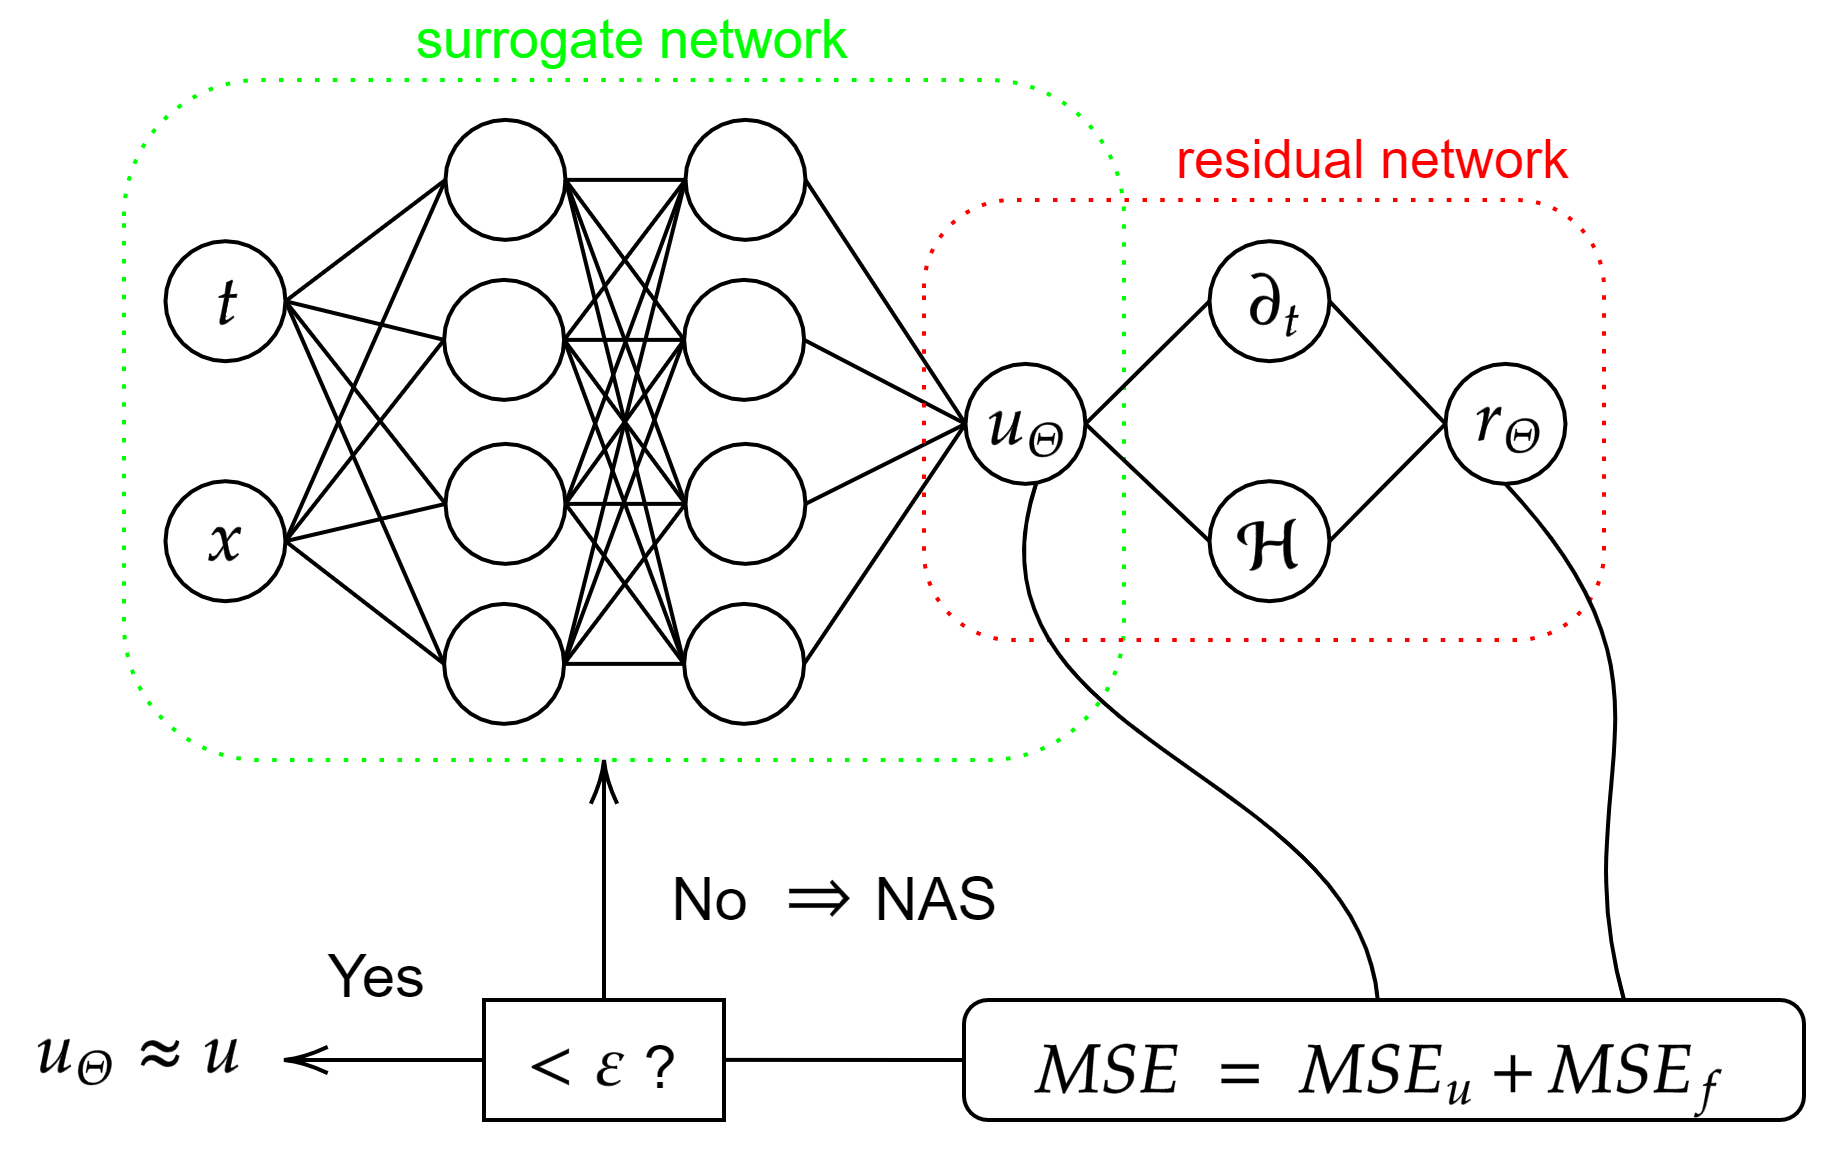
\includegraphics[scale=0.3]{img/diagram-20220212.png}
    \end{center}
    \caption{An illustration of a PINN to solve a problem with the governing differential equation \cref{PINN PDE}. The PINN consists of two basic interconnected networks. The first network (with green frame) illustrates the surrogate network $u_\Theta(t,x)$, which should approximate the solution $u$ and therefore takes the same input. This network weights and biases are trainable. The second network (with red frame) illustrates the residual network $r_\Theta(t,x)$, which takes the approximate solution from the surrogate network $u_\Theta(t,x)$ and computes the residual using automatic differentiation. The residual $r_\Theta(t,x)$ is used in a cost function to train the first network. The residual network includes the governing differential equation.}
    \label{fig6}
\end{figure}

PINNs are deep-learning networks that have to be trained. However, the residual network $r_\Theta$, which is the characteristic feature of PINNs, is officially not trained, since its only function is to provide the surrogate network $u_\Theta$ with the residual. The surrogate network $u_\Theta$ of a PINN is trained, which afterwards returns an approximate solution $u_\Theta$ of a differential equation for an input point $(t,x)$, which we call collocation point. The weights $W$ and biases $b$ of the surrogate network $u_\Theta$ can be learned by minimizing the following cost function
\begin{equation}
    \label{MSE PINN}
    MSE = MSE_u + MSE_r, 
\end{equation}
where
\begin{equation*}
    MSE_u = \frac{1}{N_u} \sum^{N_u}_{i = 1} \lVert u_\Theta(t^{u}_i, x^{u}_i) - u_i \rVert^{2}_{2}
\end{equation*}
and
\begin{equation*}
    MSE_r = \frac{1}{N_r} \sum^{N_r}_{i = 1} \lVert r_\Theta (t^{r}_i, x^{r}_i) \rVert^{2}_{2}.
\end{equation*}
The data $\{t^{u}_i, x^{u}_i, u_i \}_{i = 1, \ldots, N_u}$ denotes the initial and boundary training data on $u_\Theta$. It ensures with minimizing $MSE_u$ that $u_\Theta$ takes over the initial and boundary conditions of the differential equation. The data is generated by using, for example, for $u_i$ the value $u(0,x^{u}_i)$ explicitly required by an initial condition for all points $x^{u}_i \in \Omega$, i.e. $t^{u}_i = 0$ for all $i = 1, \ldots, N_u$. With the collocation points $\{t^{r}_i, x^{r}_i \}_{i = 1, \ldots, N_r}$, the structured information imposed by the partial differential equation is to be enforced by $MSE_r$. We note that of course the value of $MSE$ also depends on both the size of the data sets, i.e. $N_u + N_r$, and the distribution of collocation points $\{t^{r}_i, x^{r}_i \}_{i = 1, \ldots, N_r}$ (with that $\{t^{u}_i, x^{u}_i \}_{i = 1, \ldots, N_u}$). One of the most used data set distributions is the uniform distribution, where the collocation points are uniformly spaced on $\left[ 0, T \right] \times \Omega$ as on a uniform grid. In addition, simulation or experimental data can also flow in for training the network in a supervised manner, which is for example necessary for data assimilation, inverse problems and super-resolution. We see that the learning of the network $u_\Theta$, which is done by minimizing \cref{MSE PINN}, follows both a supervised approach through $MSE_u$ and an unsupervised approach through $MSE_r$. We nevertheless refer to the learning of PINNs as supervised learning, since both labelled data $u_i = u(t^{u}_i, x^{u}_i)$ is used in the optimization problem and by introducing $y_i=0$ for each collocation point $\{t^{r}_i, x^{r}_i \}_{i = 1, \ldots, N_r}$, we can form a supervised learning cost function from $MSE_r$. \\
In order to minimize $MSE$ in the training phase, two minimizers in succession are typically used: first an Adam optimizer which is an extended version of stochastic gradient descent method, see e.g. \cite{KingmaBa:2017}, and after that an L-BFGS-B optimizer \cite{ByrdLuNocedalZhu:1995}, which is a limited-memory version of the BFGS method to handle bound constrained optimization problems with many variables. Both methods only require the evaluation of $MSE$ and its gradient $\nabla_\Theta MSE$ with respect to weights and biases. An L-BFGS-B method uses an approximation of the Hessian, which expresses the curvature of $MSE$ in the high-dimensional space of weights and biases, to determine the optimization direction and gives in general more accurate results. However, using an L-BFGS-B method directly without first using an Adam optimizer can quickly lead to a local minimum of $MSE$ without leaving it. Therefore, an Adam optimizer is used first to avoid local minima, and then the solution is refined by an L-BFGS-B method \cite[p.~6]{Markidis:2021}. \\
If the surrogate network $u_\Theta$ has not been sufficiently trained by the available data so that it poorly approximates the solution $u$ of \cref{PINN PDE}, which can be seen by the amplitude of the value of $MSE$ (i.e. if the value of $MSE$ is very large, then $u_\Theta$ approximates the solution $u$ in general poorly), then the choice of the topology or the activation functions or even the choice of the type of neural network should be reconsidered. This again belongs to the task area of the NAS or the hyperparameter optimization. After a PINN is trained successfully (this can be measured by $MSE < \varepsilon$, for example), the surrogate network $u_\Theta$ can predict an approximate solution $u_\Theta (t,x)$ to the governing differential equation \cref{PINN PDE} for each point $(t,x) \in \left[ 0, T \right] \times \Omega$. Thus, it is a gridless method as any point can be taken without the need to define a grid. Moreover, the trained surrogate network $u_\Theta$ can be used to predict values on grids with different resolutions without having to be re-trained. For this reason, the computational cost does not depend on the number of grid points as in many traditional computational methods \cite[p.~2]{Markidis:2021}. \\
Although the idea of PINNs is still quite young, there are already several PINN frameworks with different network architectures for different PDE solutions. For example, \lstinline!fPINN! (fractional PINN), see \cite{PangLuKarniadakis:2019}, where the residual network is able to compute the residuals of the governing equations including fractional calculus operators, or \lstinline!vPINN! (variational PINN), see \cite{KharazmiZhangKarniadakis:2019}, where the residual network incorporates the variational form of the problem into the loss function \cite[pp.~5-6]{Markidis:2021}. All major PINN frameworks are written in \lstinline!Python!, \cite{Python}, and are based on either \lstinline!TensorFlow!, \cite{TensorFlow}, or \lstinline!PyTorch!, \cite{PyTorch}, to express the neural network architecture and to use automatic differentiation for defining the residual network \cite[p.~6]{Markidis:2021}. 